\section{Partie 1}

\subsection{Cross-Validation with GridSearchCV}
\textbf{{Question}: Explain in your report what happens when we run clf.fit(X\_train, Y\_train). What is the complexity for each of the three following cases?} \\
The line clf.fit(X\_train, Y\_train) here uses the fit method on the object  clf and taking the train sample. We give the features X and the outputs Y. The object clf is from the class GridSearchCV which allows us to find the best hyperparameters among a list we chose. It is taking as parameter an object named knn of the class KNeighborsClassifier(), a dictionary named parameters containing the number of neighbors to be tested in the knn algorithm (1 to 5 here) and the cv parameter referring to the number of folds to be used in the cross-validation. Basically it will perform a 3-folds cross-validation on a kNN model with 1 to 5 neighbors on the train sample and it will allow us to keep the best model. The kNN algorithm is parametered with the default metric which is the Euclidean distance : $\sqrt{\sum^n_{i=1}(x_i - y_i)^2}$. The functions are all part of the sklearn package. \\

\textbf{{Question}:What is the test accuracy? What would be the accuracy of random guess?} \\
The test accuracy is the measure of how often the points are correclty classified. In our case the accuracy is 0.875.  It means that 87.5\% of the time, the points are correctly classified on the test sample. If we did a random guess we would randomly choose an output in the range 0 to 9 so the accuracy would converge towards $\frac{1}{10}$ according to the LLN.  \\


\textbf{{Question}:  What is LinearSVC() classifier? Which kernel are we using? What is C? (this is a tricky question, try to find the answer online )}\\
LinearSVC means Linear Support Vector Classification. We are using a linear kernel. The parameter C represents the regularization weights, ie the penalty applied on the loss function. The loss function used here is the Squared Hinge Loss : $l(y)=\max(0,1-t\cdot y)$ \\

\begin{figure*}[ht]
	\centering 
	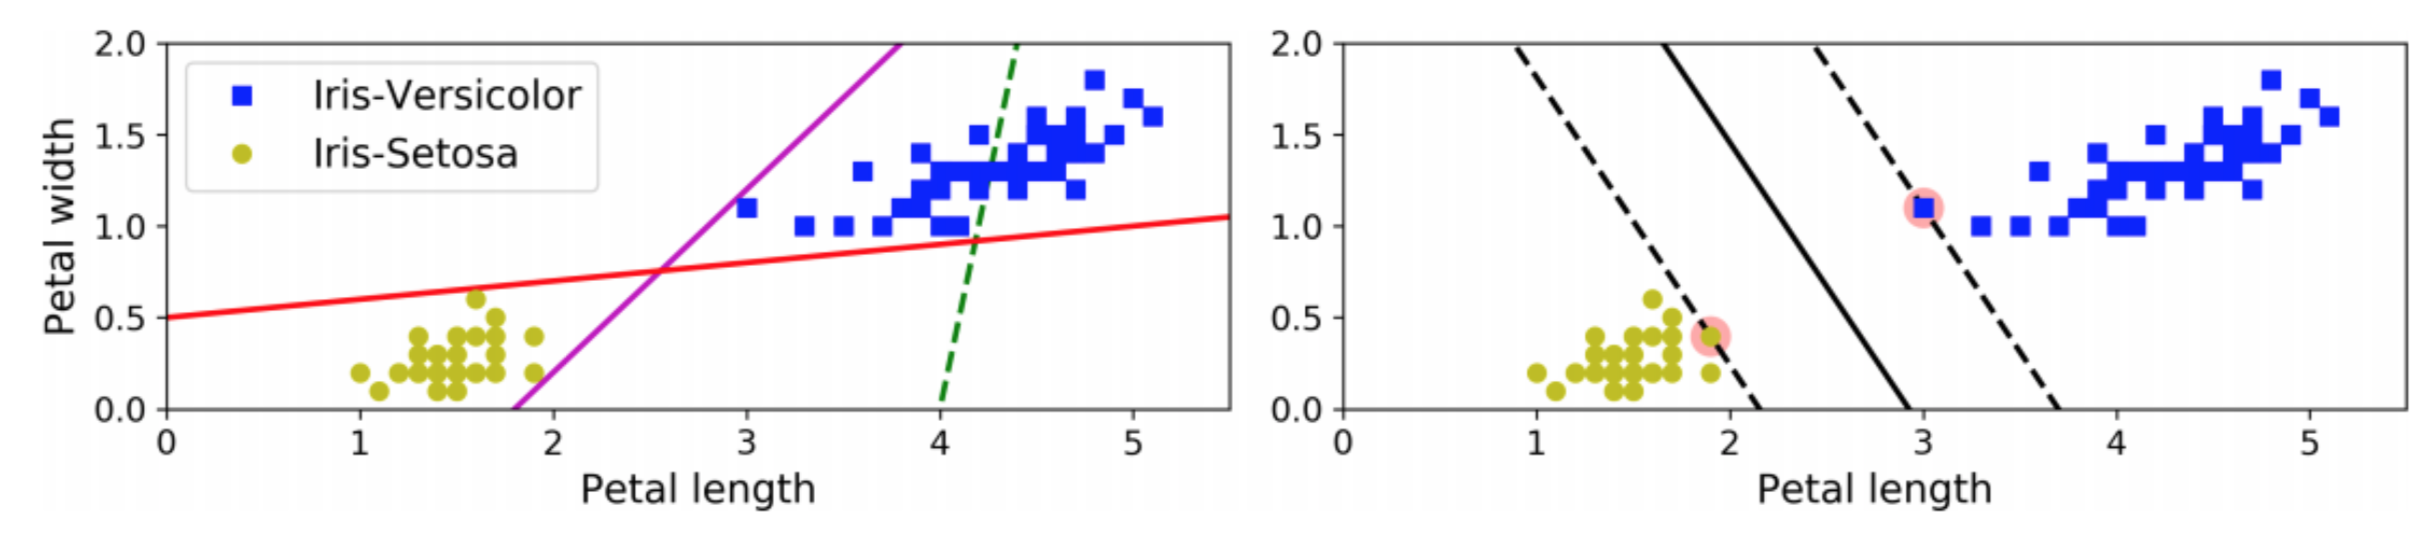
\includegraphics[scale = 0.35]{Pics/SVM}
	\caption{Example SVM}
\end{figure*}

\textbf{{Question} : What is the outcome of np.logspace(-8, 8, 17, base=2)? More generally, what is the outcome of np.logspace(-a, b, k, base=m)?}\\
The outcome of np.logspace(-8, 8, 17, base=2) is a logarthmic space going from $2^{-8}$ to $2^8$ with 17 numbers equally spaced on log scale.
 The logspace function from the numpy package will return k numbers going from $m^{-a}$ to $m^b$ spaced on a log scale with a log base m. \\

\textbf{Question : What is the meaning of the warnings? What is the parameter responsible for its appearence?}\\
The warning tells us that the algorithm did not converge, it did not reach the stop criterion. The parameter responsible for its appearence is the max\_iter parameter. Its value is not sufficient for the algorithm to converge. The data variance is maybe too large for the algorithm to efficiently perform the SVM. \\

\underline{Question} : What did we change with respect to the previous run of LinearSVC()? \\
\underline{Answer}: We added a parameter MaxAbsScaler() to scale the absolute data between 0 and 1 and thus reduce the variance. \\

\underline{Question} : Explain what happens if we execute \\
\underline{Answer}: Those lines will execute a SVM with a maxabsscaler parameter but with no C parameter which is by default 1.0.\\

\underline{Question} : what is the difference between StandardScaler() and MaxAbsScaler()? What are other scaling options available in sklearn? \\
\underline{Answer}: StandardScaler will normalize the data : $\frac{x-m}{\sigma}$ with m the mean and $\sigma$ the standard deviation of data. It differs from StandarScaler because absolute values are mapped in the range [0,1]. \\

\underline{Question} : Using the previous code as an example achieve test accuracy  $\geq0.9$ . You can use any method from sklearn package. Give a mathematical description of the selected method. Explain the range of considered hyperparamers.\\
\underline{Answer}: choose an algorithm and test \\

\subsection{Visualizing errors}
The Logistic Regression function from skLearn package is able to give us the probabilities of each outcome. The figure \ref{fig:probas} shows pictures, outcome, real value and probabilities for the 4 first mistakes, ie the 4 first times the predicted value is not equal to the real value. \\
 
\begin{figure*}[ht]
	\centering 
	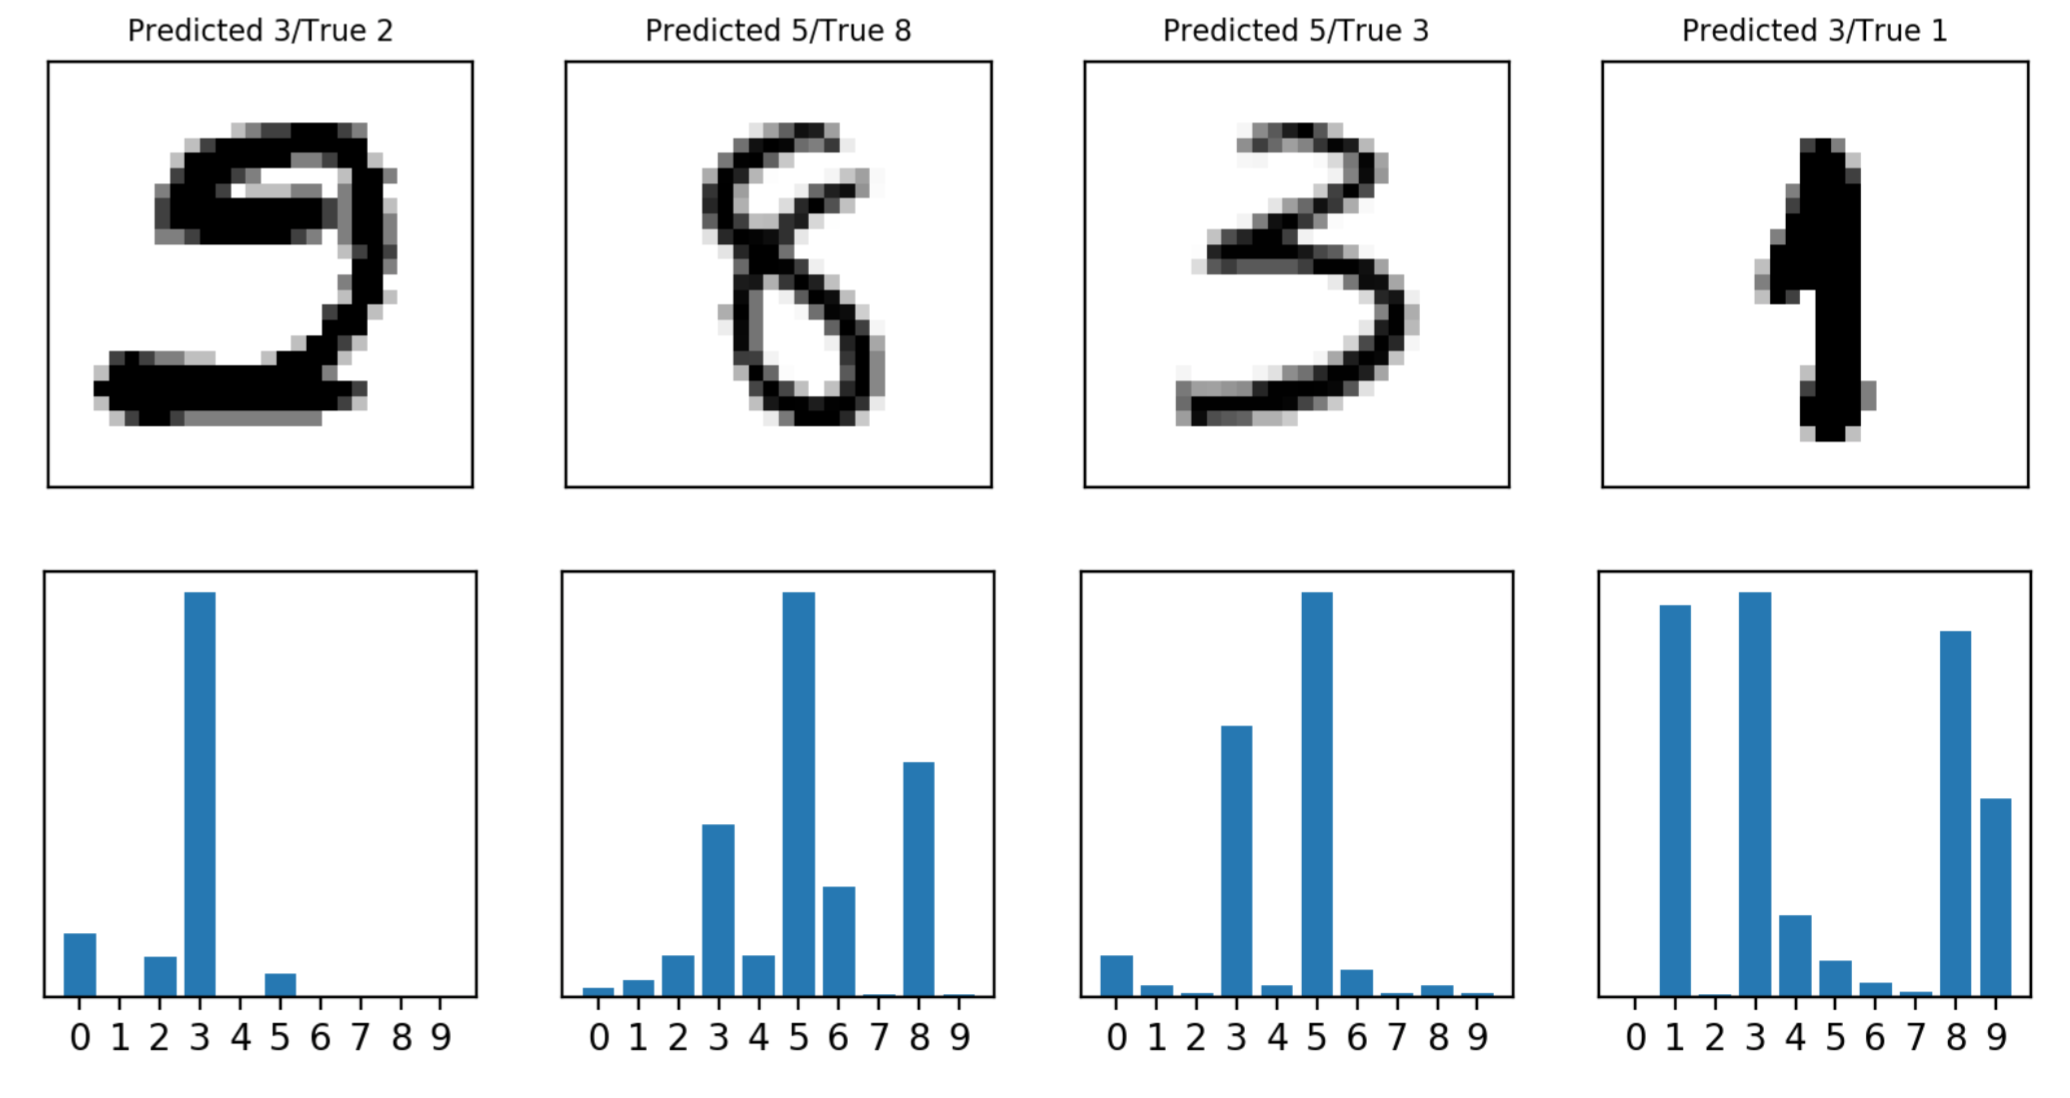
\includegraphics[scale=0.4]{Pics/probas}
	\caption{Probabilities of each outcome for the logistic regression}
	\label{fig:probas}
\end{figure*}

The error in the chunk of code was because the predict\_proba method returns an array of probabilities within an array. We must then pick the first element of the array (index 0) to obtain the proabilities array (see line 11).\\

The code is as follows :
 
\begin{lstlisting}[language=Python]
axes = plt.subplots(2, 4)[1]  # creates a grid of 10 plots

# More details about zip() function here https://docs.python.org/3.3/library/functions.html#zip
y_pred = clf4.predict(X_test)
j = 0 # Index which iterates over plots
for true_label, pred_label, image in list(zip(y_test, y_pred, X_test)):
    if j == 4: # We only want to look at 4 first mistakes
        break
    if true_label != pred_label:
        # Plotting predicted probabilities
        axes[1, j].bar(np.arange(10), clf4.predict_proba(image.reshape(1, -1))[0]) 
        axes[1, j].set_xticks(np.arange(10))
        axes[1, j].set_yticks([])
        
        # Plotting the image
        axes[0, j].imshow(image.reshape((28, 28)), cmap=plt.cm.gray_r, interpolation='nearest')
        axes[0, j].set_xticks([])
        axes[0, j].set_yticks([])
        axes[0, j].set_title('Predicted {}'.format(pred_label)+'/True {}'.format(true_label),fontsize=8)
        j += 1
\end{lstlisting}

\subsection{Changing the loss function}
 
\textbf{Question: What is balanced\_accuracy\_score? Write its mathematical mathematical description.} \\
balanced\_accuracy\_score is a method from the sklearn package that 